\documentclass[11pt, addpoints, answers]{exam}

\usepackage{amsmath, amssymb}
\usepackage{xcolor}
\usepackage{enumerate}
\usepackage{graphicx}
\usepackage{tabularx}
\usepackage{algorithm}
\usepackage{algpseudocode}
\usepackage{tikz}
\usepackage{tikz-qtree}
\usepackage{subfigure}
\usetikzlibrary{positioning}
\usetikzlibrary{graphs}
\usetikzlibrary{arrows.meta}

\newcommand{\red}[1]{\textcolor{red}{#1}}
\newcommand{\blue}[1]{\textcolor{blue}{#1}}

% For inserting code snippets.
\usepackage{listings}
\lstset{
    columns = fixed,
    numbers=left,
    basewidth = {0.5em},
    breaklines = true,
    backgroundcolor = \color{white},
    keywordstyle = \color[RGB]{40, 40, 255},
    numberstyle = \footnotesize\color{darkgray},
    commentstyle = \ttfamily\color{violet},
    basicstyle = \ttfamily,
    stringstyle = \ttfamily\color[RGB]{128, 0, 0},
    showstringspaces = false,
    language = {[11]C++},
    escapechar = \@
}
\lstnewenvironment{cpp}[1][]{\lstset{language = {[11]C++}, #1}}{}

\renewcommand{\baselinestretch}{1.15}
\setlength{\parskip}{1.25\baselineskip}

\usepackage{tikz}
\usepackage{tikz-qtree}
\tikzset{every tree node/.style={minimum width=2em,draw,circle},
    blank/.style={draw=none},
    edge from parent/.style=
    {draw,edge from parent path={(\tikzparentnode) -- (\tikzchildnode)}},
    level distance=1.2cm}


% headers, footers, titles
\newcommand{\CourseName}{CS101 Algorithms and Data Structures}
\newcommand{\HomeworkNO}{10}
\newcommand{\DueDate}{December 13, 2024}

\pagestyle{headandfoot}
\runningheadrule
\runningheader{CS101 Fall24}{Homework \HomeworkNO}{Due on: \DueDate}
\runningfooter{}{\thepage}{}

\title{
    \vspace{25pt}
    \LARGE ShanghaiTech University \\
    \bigskip
    \textbf{\CourseName} \\
    \textbf{Fall 2024}   \\
    \bigskip
    Homework \HomeworkNO
}
\author{}
\date{Due date: \DueDate, at 23:59}

% formats of questions, choices, points, etc.
\qformat{\bf\thequestion. (\totalpoints\ points) \thequestiontitle\hfill}
\pointname{'}
\CorrectChoiceEmphasis{\bf\color{blue}}
\SolutionEmphasis{\color{blue}}

% We frequently use this font.
\newcommand{\ttt}{\texttt}
\newcommand{\bluett}[1]{\textcolor{blue}{\ttt{#1}}}

\newcommand*{\TrueFalse}[1]{%
\ifprintanswers
    \ifthenelse{\equal{#1}{T}}{
        \hfill \parbox[t]{1.50in}{\begin{oneparcheckboxes} \CorrectChoice True \choice False \end{oneparcheckboxes}}
    }{
        \hfill \parbox[t]{1.50in}{\begin{oneparcheckboxes} \choice True \CorrectChoice False \end{oneparcheckboxes}}
    }
\else
    \hfill \parbox[t]{1.50in}{\begin{oneparcheckboxes} \choice True  \choice False \end{oneparcheckboxes}}
\fi
}


\begin{document}

\maketitle

\vspace{50pt}

\begin{enumerate}
    \item Please write your solutions in English.
    \item Submit your solutions to Gradescope.
    \item Set your FULL name to your Chinese name and your STUDENT ID correctly in Gradescope account settings.
    \item If you want to submit a handwritten version, scan it clearly. \ttt{CamScanner} is recommended.
    \item We recommend you to write in \LaTeX.
    \item When submitting, match your solutions to the problems correctly.
    \item No late submission will be accepted.
    \item Violations to any of the above may result in zero points.
\end{enumerate}
\newpage

\begin{questions}


\titledquestion{Multiple Choices}

Each question has \textbf{one or more} correct answer(s). Select all the correct answer(s). For each question, you will get 0 points if you select one or more wrong answers, but you will get 1 point if you select a non-empty subset of the correct answers.

Write your answers in the following table.

%%%%%%%%%%%%%%%%%%%%%%%%%%%%%%%%%%%%%%%%%%%%%%%%%%%%%%%%%%%%%%%%%%%%%%%%%%%
% Note: The `LaTeX' way to answer a multiple-choice question is to replace `\choice'
% with `\CorrectChoice', as what you did in the first question. However, there are still
% many students who would like to handwrite their homework. To make TA's work easier,
% you have to fill in your selected choices in the table below, no matter whether you use 
% LaTeX or not.
%%%%%%%%%%%%%%%%%%%%%%%%%%%%%%%%%%%%%%%%%%%%%%%%%%%%%%%%%%%%%%%%%%%%%%%%%%%

\begin{table}[htbp]
	\centering
	\begin{tabular}{|p{2cm}|p{2cm}|p{2cm}|p{2cm}|p{2cm}|}
		\hline 
		(a) & (b) & (c) & (d)  \\
		\hline
  		%%%%%%%%%%%%%%%%%%%%%%%%%%%%%%%%%%%%%%%%%%%%%%%%%%%%%%%%%%
		% YOUR ANSWER HERE.
		   &  &  &  \\
            %%%%%%%%%%%%%%%%%%%%%%%%%%%%%%%%%%%%%%%%%%%%%%%%%%%%%%%%%%
		\hline
	\end{tabular} 
\end{table}

\begin{parts}


\part[2] Which of the following statements about topological sort is/are true?
\begin{choices}
    \choice A sub-graph of a DAG may not have a topological sorting.
    \choice Any directed tree has a topological sorting.
    \choice It's possible for a DAG to have multiple topological sortings.
    \choice Since we have to scan all vertices to find those with zero in-degree in each iteration, the run time of topological sort is $\Omega(|V|^2)$.
    
\end{choices}

\part[2] Which of the following statements about topological sort is/are true?

\begin{choices}

\choice For a connected graph, we can determine if it has a cycle in $\Theta(|E|)$ time.

\choice A critical path in a DAG is a path from the source to the sink with the maximum total weights.

\choice A DAG with all different weighted edges has one unique critical path.


\choice A DAG has at least one source and at least one sink.


\end{choices}

\part[2] Which of the following sequences is/are \textbf{Topological Sorting}(s) of the given DAG?
	\vspace{0.1in}
	\begin{center}
		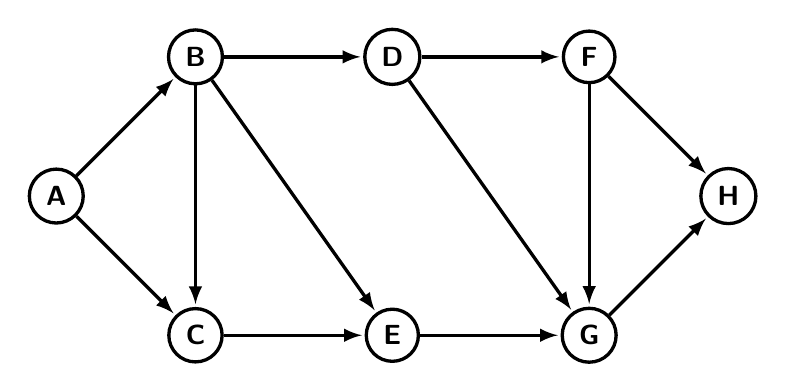
\begin{tikzpicture} [node distance = 2.5cm, very thick, main/.style = {draw, circle, font=\sffamily\bfseries}, edge/.style={->,> = latex, shorten > = 1pt}]
			\node[main] (B) {B};
                \node[main, below left of = B] (A) {A};
			\node[main, below  right of = A] (C) {C};
			\foreach \i\j in {B/D, D/F, C/E, E/G} {
					\node[main, circle, right of = \i] (\j) {\j};
				}
                \node[main, below right of = F] (H) {H};
			\draw[edge] (A) -- (B);
			\foreach \i\j in {B/C, A/C, B/D, D/F, C/E, E/G, B/E, D/G, F/H, G/H} {
					\draw[edge] (\i) -- (\j);
				}
			\draw[edge] (F) -- (G);
		\end{tikzpicture}
	\end{center}
	\begin{choices}
    	\choice 	    A B C E G D F H
		\choice 	A B C D E F G H
		\choice 	A B D C F E G H
		\choice 	    A B D E C F G H
	\end{choices}

\part[2]For the coin-changing problem, denote
    \begin{itemize}
        \item $C=(c_1, c_2,\cdots,c_k)$: the denominations of coins, where $1=c_1<c_2<\dots<c_k$;
        \item $X_n^*$: an optimal solution, i.e., a multi-set of coins which has the minimum number of coins to make change for $n$;
        \item $X_n$: the greedy solution, solved by
        \[
        X_n=\begin{cases}
        \{ \},&n=0\\
        \{c_t\}\cup X_{n-c_t},&n\ge 1, \text{where } c_t=\max\limits_{c_i\le n}c_i \text{ is the largest coin that can be used}
        \end{cases}
        \]
    \end{itemize}

For example, if $C=(1,2,3)$, then $X_4^*$ can be either $\{2,2\}$ or $\{3,1\}$, and $X_4=\{3,1\}$.

Which of the following statements is/are true?

    \begin{choices}
 
        \choice If $\forall i\in[3,n], c_i=c_{i-1}+c_{i-2}$, then $\forall n,|X_n^*|=|X_n|$.
        \choice $\exists C,\exists i$ with $2c_i>c_{i+1}$, such that $\forall n,|X_n^*|=|X_n|$.
        \choice If $\forall i, 2c_i\le c_{i+1}$, then $\forall n,|X_n^*|=|X_n|$.
        \choice If $\forall i\in[2,n], \dfrac{c_i}{c_{i-1}}$ is an integer, then $\forall n,|X_n^*|=|X_n|$.
 
    \end{choices}

\end{parts} 

\newpage

\titledquestion{A star}

Logan is doing an A* \textbf{graph search} from $S$ to $T$ on the graph below. Edges are labeled with weights.

The exploration order follows in their lexicographical order. (For example, $S \to X \to A$ would be expanded before $S \to X \to B$, and $S \to A \to Z$ would be expanded before $S \to B \to A$.
\begin{table}[!ht]
\begin{minipage}[b]{0.6\linewidth}
\centering
    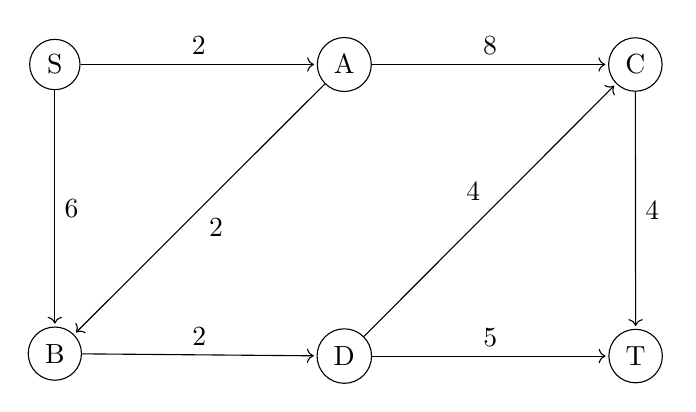
\begin{tikzpicture}[shorten >=1pt,node distance=2cm,auto]
    \node[circle,draw] (S) {S};
    \node[circle,draw] (A) [right=3cm of S] {A};
    \node[circle,draw] (B) [below=3cm of S] {B};
    \node[circle,draw] (C) [right=3cm of A] {C};
    \node[circle,draw] (D) [below=3cm of A] {D};
    \node[circle,draw] (T) [right=3cm of D] {T};
    \path[->]
    (S) edge node {2} (A)
    (A) edge node {2} (B)
    (S) edge node {6} (B)
    (B) edge node {2} (D)
    (D) edge node {5} (T)
    (A) edge node {8} (C)
    (D) edge node {4} (C)
    (C) edge node {4} (T);
\end{tikzpicture}
\end{minipage}
    \begin{minipage}[b]{0.35\linewidth}
    \centering
    \begin{tabular}{|r|l|l|l|l|l|l|}
    \hline
        Node & S & A & B & C & D& T \\ \hline
        Heuristic & $11$ & $9$ & $12$ & $4$ & $5$ & $0$ \\ \hline
    \end{tabular}
    \caption{The initial heuristic value}
    \label{tab:heuristic}
    \begin{table}[H]
    \centering
    \begin{tabular}{|r|l|l|l|l|l|l|}
    \hline
        Node & S & A & B & C & D& T \\ \hline
        Heuristic & $10$ & $6$ & $4$ & $2$ & $3$ & $0$ \\ \hline
    \end{tabular}
    \caption{The new heuristic value}
    \label{tab:new}
    \end{table}
\end{minipage}
\end{table}\\

\begin{parts}
    \part[3] He first uses the heuristic value in the Table \ref{tab:heuristic} but finds it does not work well. That's because the given heuristic values are:
\begin{choices}
    \choice Admissible but not consistent
    \choice Consistent but not admissible
    \choice Neither admissible nor consistent
\end{choices}
\part Logan decides to modify the heuristic.
\begin{subparts}
    \subpart[3] He first gives out a new heuristic as in Table \ref{tab:new} above, please check whether the heuristic meets both admissibility and consistency (Write `Yes' or `No' for this). \\
    \textbf{If so}, write down the path from $S$ to $T$ returned by $A^*$ graph search (in the form of nodes, e.g. $S\to A \to C \to T$ should be written as $SACT$). \\
    \textbf{Otherwise}, give out a contradiction that will lead admissibility or consistency to fail (in the form of `Admissibility/Consistency' and its corresponding inequality. \\
    e.g. If consistency fails on $A\to C$, write `Consistency, $h(C) + 8 < h(A)$', here $8$ corresponds to $w(A, C)$.).
\begin{solution} \\
    \vspace{2in}

\end{solution}
    \subpart[4] He finds that he can modify the heuristic of \textbf{only one node} to meet admissibility and consistency from the initial heuristic values in Table \ref{tab:heuristic}. Find the node and corresponding heuristic value for the chosen node. Justify your answer by stating the equalities obtained from admissibility and consistency.
\begin{solution} \\
    \vspace{2in}

\end{solution}
\end{subparts}

\end{parts}
\titledquestion{The shortest path with vertex weights}[10]

Given a directed graph $G = (V, E)$, you need to find the path from $s$ to $t$ with minimum cost. The edges are not weighted i.e. you can regard them as $1$. However, the vertices in $V$ have their weights and those are required to be considered in the path.

The graph $G = (V, E)$ is
\begin{itemize}
    \item $V=\{1,2,\ldots, n\}$, where each vertex $i$ is associated with a positive vertex weight $a_i > 0$,
    \item $E=\{(u_i,v_i):i=1,2,\ldots, m\}$, where each edge $(u_i, v_i)$ is associated with a positive edge weight $1$.
    % \item The start point $s$ and the end point $t$.
\end{itemize}
And $F: V\to \mathbb{R}^+$ represents the weight assigning function. (e.g. weight of vertex $u$ is $F(u)$.)

A path is defined as a series of vertices $v_0\to v_1\to \cdots\to v_k$, which involves $k$ edges and satifies that $\forall\ 0\leq i <k, ((v_i,v_{i+1})\in E)$ (which implies $\forall\ 0\leq i \leq k, v_i\in V$.).

The cost $C(P)$ of path $P = v_0 \to v_1 \to \cdots \to v_k$ is as follows:
\begin{align*}
    C(P) = \sum_{i=0}^k F(u_i) + k
\end{align*}

Now given a vertex $s\in V$, you need to find path $P = s \to (v_1 \to \cdots ) \to t$ with minimum cost for all $t \not = s$.
You are supposed to give out the $|V|-1$ minimum cost of the paths. Guaranteed that $s$ can reach all other vertices.

You should give out the steps of your algorithm (\textbf{as efficient as possible}) together with the time complexity (tight). You don't need to prove the correctness of your algorithm.


\textbf{Hint:} Try to create a new graph instead of modifying the algorithm known.
\begin{solution} \\
    \vspace{2in}

\end{solution}
\titledquestion{Negative Cycle Detection}
The \textbf{inf($\infty$)} mentioned in this problem could be regarded as a pre-defined large enough constant. The graph mentioned in this problem is a simple directed graph. Please write down your codes in \textbf{standard C++}.

\begin{parts}
\part Consider the following implementation of the Floyd-Warshall algorithm. Suppose $W$ is the adjacency matrix of the graph, and assume that $W_{ij}=\infty$ where there is no edge between vertex $i$ and vertex $j$, and assume $W_{ii}=0$ for every vertex $i$. And other $W_{ij}$ are the weights of the edge between vertex $i$ and vertex $j$.  The array `graph' passed into the function is the adjacency matrix $W$.

\begin{cpp}
bool DetectNegCycle_Floyd(const int graph[][V])
{
    int dist[V][V];

    for (int i = 0; i < V; ++i)
        for (int j = 0; j < V; ++j)
            dist[i][j] = graph[i][j];

    for (int k = 0; k < V; ++k)
        for (int i = 0; i < V; ++i)
            for (int j = 0; j < V; ++j)
                if (dist[i][j] > dist[i][k] + dist[k][j])
                        dist[i][j] = dist[i][k] + dist[k][j];

    _____________________________________
    _____________________________________
    _____________________________________
    _____________________________________

    return false;
}
\end{cpp}

\begin{subparts}

\subpart [2] Consider the three loop lines in the Floyd-Warshall algorithm: lines $9, 10$, and $11$. Which pair(s) of these lines can be swapped without affecting the correctness of the algorithm? List all possible pairs of lines that can be swapped.

\begin{solution} \\
    \vspace{2in}

\end{solution}

\subpart[4] Add some codes in the blank lines to detect whether there are negative cycles in the graph. (You may not use all blank lines, or you can add more lines.)

\begin{solution}
\begin{cpp}
    _____________________________________
    _____________________________________
    _____________________________________
    _____________________________________
\end{cpp}
\end{solution}
\end{subparts}

\part[4] Consider the following implementation of the Bellman-Ford algorithm. The `edge' structure is used to represent the edges of the graph, with its elements $u$, $v$, and $w$ denoting an edge from node $u$ to node $v$ and its corresponding weight $w$.

\begin{cpp}
struct edge
{
    int u, v, w;
};

bool detectNegCycle_BellmanFord(const std::vector<edge>& Edge, int s)
{
    int dist[V];

    for (int i = 0; i < V; ++i)
        dist[i] = inf;
    dist[s] = 0;

    for(i = 1; i <= V - 1; ++i)
    {
        for(const auto& e : Edge)
            if (dist[e.v] > dist[e.u] + e.w)
                dist[e.v] > dist[e.u] + e.w;
    }

    _____________________________________
    _____________________________________
    _____________________________________
    _____________________________________

    return false;
}
\end{cpp}

Add some codes in the blank lines to detect whether there are negative cycles in the graph. (You may not use all blank lines, or you can add more lines.)

\begin{solution}
\begin{cpp}
    _____________________________________
    _____________________________________
    _____________________________________
    _____________________________________
\end{cpp}
\end{solution}

\end{parts}
\titledquestion{Arbitrage}

\textbf{Preface:} Shortest-path algorithms can be applied to many real-life domains. One of the most challenging aspects is constructing the graph in a complex environment. Consider the scenario below:

Recently, our beloved TA, Flash, was hired by an anonymous financial firm to assist with financial oversight. At the firm, Flash has access to a set of $n$ currencies $C = {c_1, c_2, \dots, c_n}$, including US dollars, Euros, Bitcoin, Dogecoin, and others. For every pair of currencies $c_i$ and $c_j$, Flash knows the exchange rate $r_{i,j}$ which indicates how many units of currency $c_j$ you can receive in exchange for one unit of currency $c_i$. Assume that $r_{i, i} = 1$ for all currencies and that $r_{i, j} > 0, r_{i,j} = \dfrac{1}{r_{j,i}}$ for all pairs $i, j$.

Since the exchange rates between different currencies can be volatile and unpredictable, there may be times when you can start with one unit of arbitrary currency $c_i$ and end up with more than one unit of $c_i$ through exchanging. Such a situation is known as \textbf{arbitrage}.

More formally, arbitrage occurs if there exists a sequence of currencies $c_{i_1}, c_{i_2}, \dots, c_{i_k}$ such that:
$$ r_{i_1, i_2} \cdot r_{i_2, i_3} \cdot \cdots \cdot r_{i_{k-1}, i_k} \cdot r_{ik, i_1} > 1 $$

A system of exchange rates is considered \textbf{arbitrage-free} if there is no such sequence of exchanges that results in a profit, i.e. it is impossible to gain more than one unit of any currency by performing a series of exchanges.

Due to his heavy TA workload, Flash needs your help to design algorithms that can efficiently perform the tasks assigned by the company.

\begin{parts}
\part[5] Flash has access to a set of exchange rates of $(r_{i,j})_{i,j \in {1, 2, \dots, n}}$, his first task is to find the most profitable sequence between currencies $a$ and $b$. In other words, given a fixed amount of currency $a$, he can get the most amount of currency $b$ through this sequence of exchanges.
\textbf{In this part, suppose the set of exchange rates is arbitrage-free.}

To assist Flash, please provide your algorithm and analyze the time-cost of it. You don't need to prove the correctness of the algorithm. Your time complexity should not exceed the complexity of the algorithms taught in the current course.

\textbf{Hint:} $\log(xy) = \log(x) + \log(y)$.

\begin{solution} \\
    \vspace{2in}

\end{solution}


\part[5] The second task of Flash is to detect whether arbitrage exits given an exchange rate set at any specific time, which is, obviously, too hard to do manually.

For this part, please give your algorithm, analyze its time complexity, and briefly explain why it can work. Your time complexity should not exceed the complexity of the algorithms taught in the current course.

\end{parts}

\begin{solution} \\
    \vspace{2in}

\end{solution}
\titledquestion{k-layer Shortest Path}

Consider a weighted directed graph $ G = (V, E) $ and source vertex $ s \in V $. It is given that for each vertex $ v \in V $, there exists a shortest path from $ s $ to $ v $ that uses at most $ k $ edges. Devise an algorithm to determine the shortest path weight from $ s $ to every vertex $ v \in V $.

\textbf{Hints}: \textit{Consider to rebuild a graph with $O(k|V|)$ number of node.}

\begin{parts}
\part[3] Design an algorithm to solve this problem using the shortest-path algorithm. Which algorithm will you choose Explain why.

\begin{solution} \\
    \vspace{2in}

\end{solution}

\part[3] As the shortest path only uses at most $k$ edges, optimize your algorithm to $ O(|V| + k|E|) $ time.

\begin{solution} \\
    \vspace{2in}

\end{solution}
\end{parts}


\end{questions}

\end{document}